\cleardoublepage
\chapter{First steps outside the Local Group of Galaxies:Red Supergiants in NGC\,55}
\label{ch:ngc55}

% \textbf{Completeness:} \textbf{30\%} \\
% The observations for this section are complete and the data reduction is
% currently being optimised.

% \textbf{Description:} \\
% This chapter will outline KMOS observations of 20 RSGs in NGC\,55.
% I will descibe the work I have done in preperation for these observations.

% I will discuss the optimisations which have been made for this data set and
% describe the challenges of obtaining the best possible data from a set of
% challenging observations.

% I will comment on the spatial distribution of the chemical abundances in this
% galaxy and discuss a potential metallicity gradient previously suggested in
% the literature.

\section{Opening Remarks} % (fold)
\label{sec:ngc55open}

To improve the quality of the data reduction I enlisted the help of a fellow student, Owen Turner, who has provided some additional corrections to the standard KMOS/esorex pipeline to correct for the readout bias and to improve the pipeline's bad pixel map.
Details of this procedure are given in the text and the reader is referred to Turner et al. (in prep) for a more in depth discussion of the steps taken.
% section opening_remarks (end)

\section{Introduction} % (fold)
\label{sec:ngc55intro}

NGC\,55 is a galaxy located outside of the Local Group of Galaxies within the Sculptor Group at a distance of 1.94\,$\pm$\,0.03\,Mpc~\citep{2006AJ....132.2556P,2008ApJ...672..266G} which, before the emergence of the Araucaria Project~\citep{2005Msngr.121...23G}, had been subject to considerable uncertainty~\citep[e.g.][]{1987ApJ...323...79P,2006A&A...455..891V}.

The Sculptor ``Group'' includes five massive galaxies (NGC\,55, NGC\,247, NGC\,253, NGC\,300 and NGC\,7793) and numerous ($\sim$20) dwarf galaxies.
NGC\,253 is a large starburst galaxy and is the brightest and most massive of the group. This is the closest group of galaxies to the Local Group, and offers a fantastic laboratory to test theories of stellar and galactic evolution as, using an 8-m class telescope, one can resolve individual stars within these galaxies.

Association to the Sculptor Group however, is a contentious issue.
By revising distances for nine of the Sculptor Group dwarfs~\cite{2003A&A...404...93K} postulated that the Sculptor group was actually more like a filament of galaxies, which intersects the Milky Way group, where NGC\,55 and NGC\,300 and their surrounding satellite galaxies were potentially not associated with the main group of galaxies in this filament.
Regardless of the geometry and association to the Sculptor Group, NGC\,55 is the nearest large galaxy to the MW group in the direction of the Sculptor Group.

The morphology of NGC\,55 is asymmetric and complicated owing to the high inclination angle~\cite[up to 80\textdegree;][]{1986A&A...166...97H,2013MNRAS.434.3511W}.
\cite{1961ApJ...133..405D} classified this galaxy as an LMC-like spiral barred galaxy (SB(s)m) where the bar is seen along the line of sight~\cite{1961ApJ...133..405D}
prompting various claims that this galaxy is an edge-on analogue of the LMC~\citep[e.g.][although not cited heavily -- two citations in 50 years -- the idea has propagated]{1964IAUS...20..276R}.
Figure~\ref{fig:ngc55-wide} shows NGC\,55 and its complicated morphology where one can see the edge-on disk along the major axis of the galaxy and the brighter central part of the galaxy represents the head of the bar.
In addition, to NGC\,55 being orientated nearly edge on, extending from the disk-bar system there exists many star-formation features such as giant H\,\2 regions as well as supergiant filaments and shells which are thought to allow ionising radiation to be transported to the halo where star-formation is currently occurring~\citep{1996AJ....112.2567F}.

\begin{figure}
 \centering
 \includegraphics[width=0.65\textwidth]{ngc55/eso0914a-v3}
 \caption[Image of NGC\,55]{Image of NGC\,55 where the edge-on disk of the galaxy makes up the major axis and the bright central region represents the head of the bar containing intense star-forming regions.
 Image from the Wide Field Imager on the 2.2-metre MPG/ESO telescope at ESO La Silla Observatory. Credit: ESO, press release.}
 \label{fig:ngc55-wide}
\end{figure}


The morphology of NGC\,55, as well as its known population of massive hot stars~\citep{2008A&A...485...41C,2012A&A...542A..79C}, points to a recent history of intense star formation.
This is supported by the infrared morphology of NGC\,55 which is dominated by young star-forming features~\citep[][with a star-formation rate of 0.22\,M$_{\odot}$yr$^{-1}$]{2004ApJS..154..248E} as well as indications from near-IR imaging~\citep{2005ApJ...622..279D}.

The metal content of NGC\,55 is expected to be LMC-like, which is supported by~\cite{2012A&A...542A..79C} who measured metallicities of 12 blue supergiants using optical spectroscopy and found a mean metallicity [Z]~=~$-$0.40\,$\pm$\,0.13\,dex.
In addition,~\cite{1983MNRAS.204..743W} measure abundances of seven H\,\2 regions across the disk of NGC\,55 using the strong-line method (as well as four measurements of the auroral ``direct'' line method) and found a similar LMC-like metallicity.

Even though the hot massive star population of NGC\,55 has been explored,
there are currently no confirmed RSGs in NGC\,55, although~\cite{2005ApJ...622..279D} note that the near-IR CMDs of fields within the disk of NGC\,55 reveal signatures of RSGs.
This study represents the first quantitative study of RSGs in NGC\,55 and, by measuring metallicities of this population, will provide a crucial test of the metallicity gradient within this galaxy.

In this chapter, I describe the observations and data reduction procedure in Section~\ref{sec:ngc55obs} and highlight the target selection method and its uncertainties.
I then present the main results of the chapter in Section~\ref{sec:ngc55results} where I first measure radial velocities for each epoch of the RGSs, confirming their membership of NGC\,55, and then go on to measure stellar parameters for each target using the $J$-band analysis technique described in detail in Chapter~\ref{ch:janal}.
The main conclusions are presented in Section~\ref{sec:ngc55conc}.

% section introduction (end)

\section{Observations} % (fold)
\label{sec:ngc55obs}

\subsection{Target Selection} % (fold)
\label{sub:target_selection}

% In order to select RSG candidates in NGC\,55 I compiled optical photometry from two sources: The Araucaria Project~\citep{2005Msngr.121...23G} and the ACS Nearby Galaxy Survey Treasury project~\citep[ANGST][]{2009ApJS..183...67D}.
% Figure~\ref{fig:ngc55-foot} displays the footprints of the two projects.

Targets were selected based on their optical photometry from the the Araucaria Project~\citep{2005Msngr.121...23G} where the footprints for this project are highlighted with large white rectangles in Figure~\ref{fig:ngc55-foot}.
The optical CMD which is used to select targets is displayed in the left hand panel of Figure~\ref{fig:VI}, where the RSG candidates are within the black box and the observed targets are highlighted in red.
This method of target selection is preferred as a result of the limited extent of near-IR photometry in this area.



\begin{figure}
 \centering
 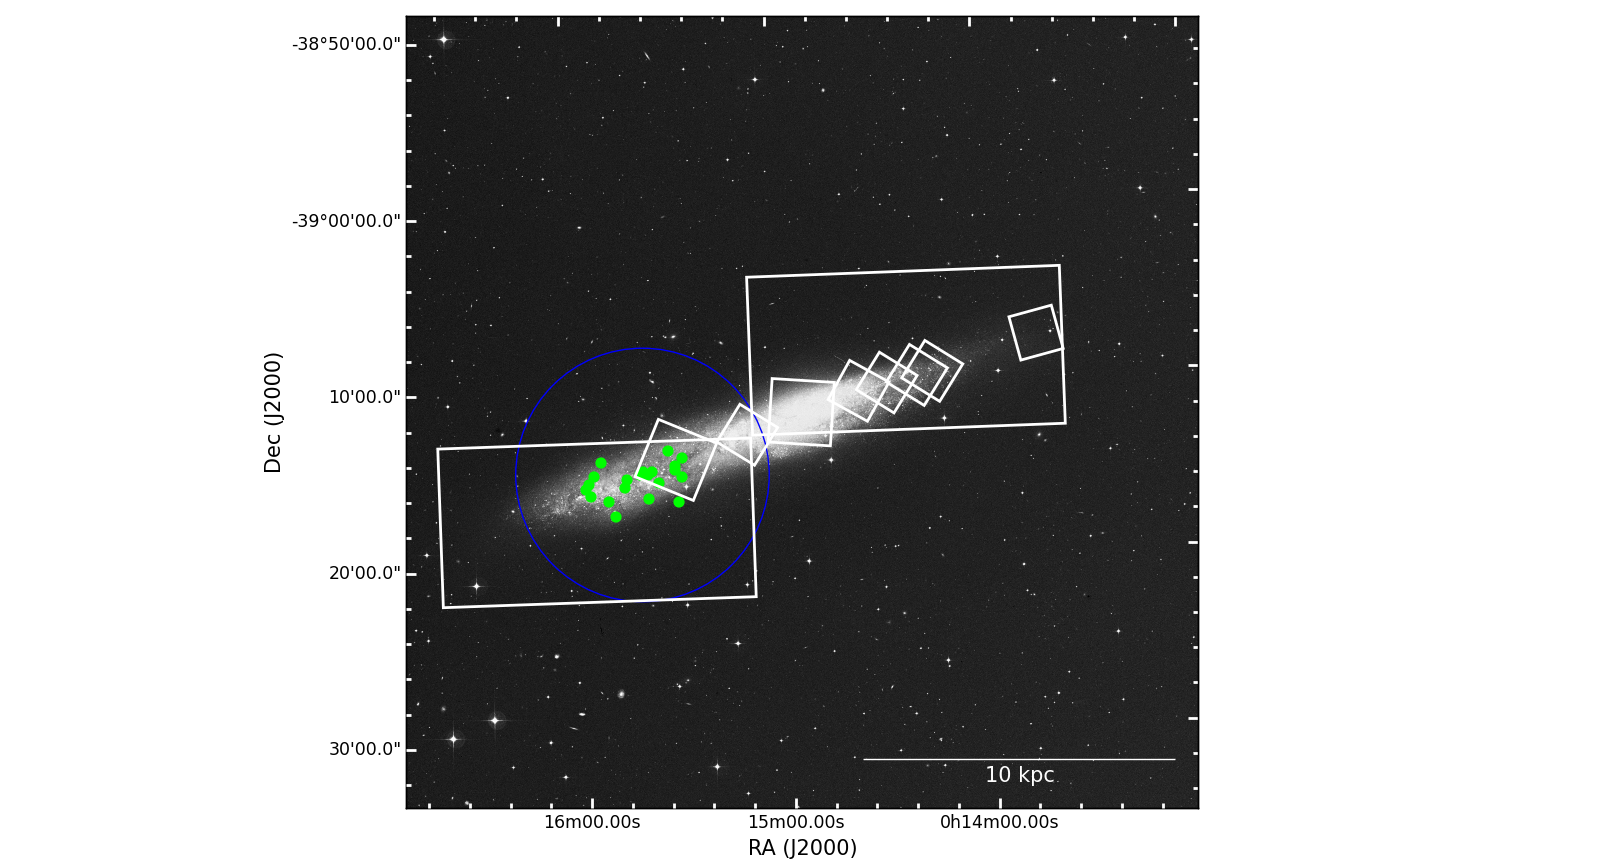
\includegraphics[width=\textwidth]{ngc55/ngc55_fields-v3}
 \caption[DSS image of NGC\,55 with KMOS and photometric footprints highlighted]{
          DSS image of NGC\,55 with KMOS targets overlaid in green and photometric footprints from the Araucaria Project
          \protect\citep{2005Msngr.121...23G} in white rectangles
          and the ANGST project
          \protect\citep{2009ApJS..183...67D} in the smaller white squares.
         }
 \label{fig:ngc55-foot}
\end{figure}


\begin{figure}
  \centering
  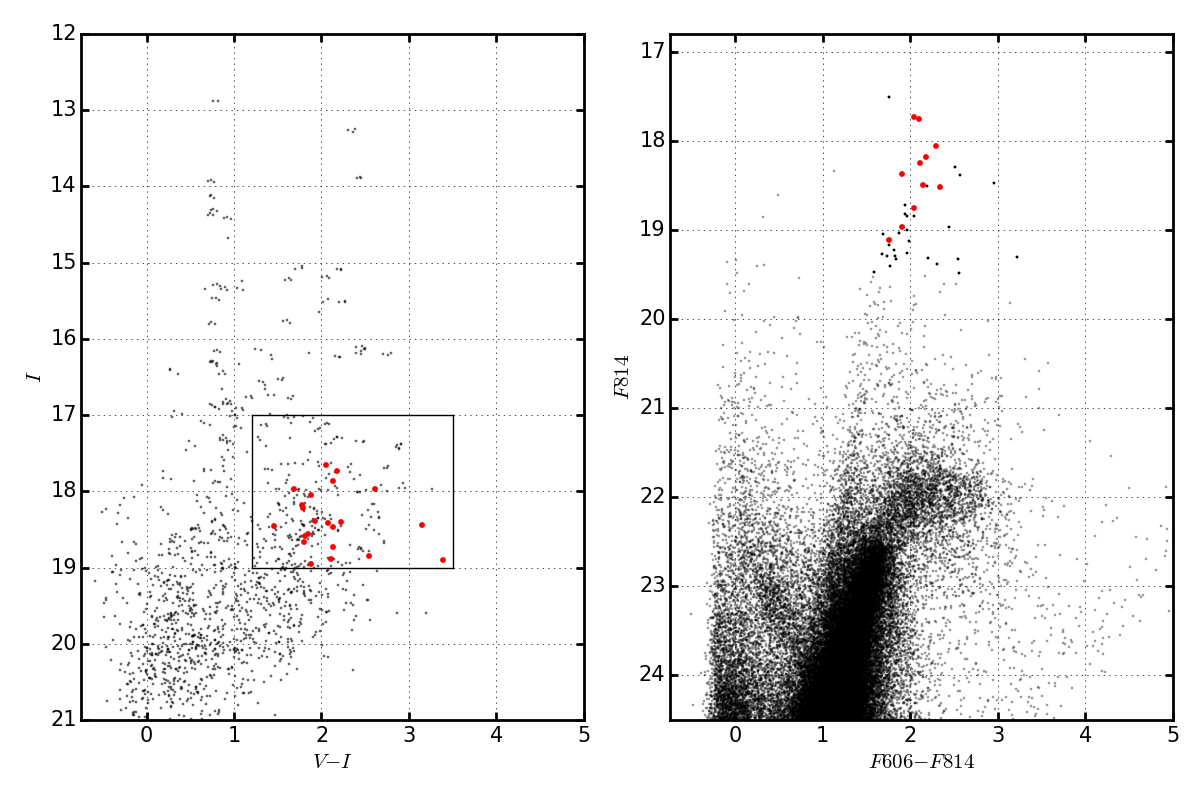
\includegraphics[width=\textwidth]{ngc55/ngc55-v_i_both}
 \caption[NGC\,55 ground- and space-based colour--magnitude diagrams]{
  NGC\,55 ground- and space-based colour--magnitude diagrams. Left hand panel shows $V-I$, $I$ data from the ground-based Araucaria Project~\cite{2005Msngr.121...23G}
  over the entire field-of-view (Fov) of the KMOS observations.
  The black box defines candidate RSGs which are defined as
  $17 < I < 19$ and $1.2 < V-I < 3.5$.
  Right hand panel shows data from the ACS Nearby Galaxy Survey Treasury
  \citep[ANGST][]{2009ApJS..183...67D} project where photometry from this project covers only a portion of the KMOS FoV (see Figure~\ref{fig:ngc55-foot}).
          }
 \label{fig:VI}
\end{figure}


Candidate RSGs, illustrated by the black box in the left hand panel of Figure~\ref{fig:VI}, are defined as $17 < I < 19$ and $1.2 < V-I < 3.5$.
The magnitude limit here is a result of to the expected magnitudes of RSGs in NGC\,55~\citep[e.g.][who identified RSGs in NGC\,300]{2015ApJ...805..182G} and the $V-I$ colour limit is chosen to avoid potential Galactic contamination at $V-I\sim$ 0.95.
All stars that meet this criteria are defined as candidate RSGs and the final target selection was performed by analysing the spatial location of the candidates and selecting those which traced the disk population of NGC\,55 (see Figure~\ref{fig:ngc55-foot}).

In addition to the ground-based photometry available, the ACS Nearby Galaxy Survey Treasury~\citep[ANGST][]{2009ApJS..183...67D} project has publicly available photometry for several fields within the disk of NGC\,55 that are displayed as small white squares in Figure~\ref{fig:ngc55-foot}.
A $F814$, $F814-F606$ CMD is shown in the right hand panel of Figure~\ref{fig:VI} for the ACS ANGST field which contains 11 of our KMOS targets, where observed KMOS targets are highlighted in red.
Given the smaller spatial coverage of the HST ACS field, the expected number of Galactic contaminants is corresponding smaller.
To add to this as a result of their cool temperatures and extreme luminosities, RSGs should exist in a ``plume'' at the tip of a structure of cool stars in the $F606-F814$, $F814$ CMD (assuming no contamination).
This compares well to the location (in colour--magnitude parameter space) of confirmed RSGs in NGC\,300~\citep{2015ApJ...805..182G}.
Therefore, all candidates with HST photometry are classified as priority one targets.


% In addition to the ANGST HST photometry, ground-based optical photometry is obtained from the Araucaria Project which covers the full spatial extent of NGC\,55 (large white rectangles in Figure~\ref{fig:ngc55-foot}).

% The selection criteria used in this study makes is based optical $F606-F814$ colours and $F814$ magnitudes.
% Owing to their cool temperatures and extreme luminosities RSGs are known to exist in a ``plume'' at the tip of a structure of cool stars in the $F606-F814$, $F814$ CMD~\citep[e.g.][]{2015ApJ...805..182G}.
% Figure~\ref{fig:VI} displays this CMD and the region of parameter space where RSG candidates reside is marked with a grey box.
% This box has the limits $17 < F814 < 19$ and $1.2 < F606-F814 < 3.5$ following~\cite{2015ApJ...805..182G}, where the faint magnitude limit is chosen to select only targets which will have a S/N~=~100 in the original observing proposal.
% As with selection criteria in the near-IR, the lower limit of this criteria is contaminated with a population of super-AGB stars which can have luminosities comparable to the faintest RSGs~\citep[e.g.][]{2000ApJ...542..804N}.
% However, as stated in Chapter~\ref{ch:n6822} these stars are known to have lifetimes similar to the lowest mass RSGs and arguably still trace the young stellar population of this galaxy.



Table~\ref{tb:n55obs-params} shows ground- and space-based optical photometry of the KMOS targets along with their radial velocities which confirm many of these targets as NGC\,55 RSGs
(see Section~\ref{sub:rvs}).



\begin{sidewaystable}
\caption[Summary of VLT-KMOS targets in NGC\,55]{Summary of VLT-KMOS targets in NGC\,55.\label{tb:n55obs-params}}
\scriptsize
\begin{threeparttable}
\centering
\begin{tabular}{lcccccccccccl}
 \hline
 \hline
ID & $\alpha$ (J2000) & $\delta$ (J2000) & $V$\tnote{a} & $I$\tnote{a} & $F606$\tnote{b} & $F814$\tnote{b} & \multicolumn{4}{c}{$rv$ (\kms)} & $\langle rv\rangle$ (\kms) & Notes \\
\cline{9-12}
& &  & & & & & & 14-09-2013 & 16-10-2013 & 14-09-2014 & 15-09-2014\\

 \hline
NGC55-RSG19 & 00:15:29.190 & $-$39:14:08.20& 19.914 & 17.731 &19.85 & 17.76 &   205\,$\pm$\,4  &  178\,$\pm$\,7   &    222\,$\pm$\,10 &   191\,$\pm$\,7               & 199\,$\pm$\,14 & \\
NGC55-RSG20 & 00:15:29.520 & $-$39:15:13.00& 20.832 & 18.952 &20.86 & 19.11 &   194\,$\pm$\,14 &  220\,$\pm$\,5   & -- & --                                           & 217\,$\pm$\,10 & \\
NGC55-RSG22 & 00:15:30.520 & $-$39:16:36.70& 20.406 & 18.589 & --   & --    &    95\,$\pm$\,14 &$-$41\,$\pm$\,26  & -- & --                                           & --             & \\
NGC55-RSG24 & 00:15:31.460 & $-$39:14:46.30& 20.612 & 18.475 &20.29 & 18.38 &   186\,$\pm$\,6  &  194\,$\pm$\,7   &    146\,$\pm$\,38 &   237\,$\pm$\,16              & 192\,$\pm$\,16 & \\
NGC55-RSG25 & 00:15:31.490 & $-$39:14:32.40& 20.316 & 18.394 &20.63 & 18.49 &   204\,$\pm$\,12 &  217\,$\pm$\,16  & $-$376\,$\pm$\,41\tnote{c} & 151\,$\pm$\,23       & 200\,$\pm$\,26 & \\
NGC55-RSG26 & 00:15:33.160 & $-$39:13:42.00& 20.572 & 17.964 &20.35 & 18.06 &   174\,$\pm$\,9  &  173\,$\pm$\,8   & -- & --                                           & 173\,$\pm$\,1  & \\
NGC55-RSG28 & 00:15:36.160 & $-$39:15:29.40& 21.001 & 18.892 &20.87 & 18.97 &   233\,$\pm$\,17 &  161\,$\pm$\,20  & -- & --                                           & 203\,$\pm$\,41 & \\
NGC55-RSG30 & 00:15:38.030 & $-$39:14:50.20& 20.867 & 18.730 &20.79 & 18.75 &   212\,$\pm$\,10 &  215\,$\pm$\,10  & $-$424\,$\pm$\,21\tnote{c} & 212\,$\pm$\,22       & 213\,$\pm$\,2  & \\
NGC55-RSG35 & 00:15:39.260 & $-$39:15:01.70& 20.007 & 17.872 &19.78 & 17.73 &   202\,$\pm$\,3  &  206\,$\pm$\,4   &    223\,$\pm$\,13 &   200\,$\pm$\,11              & 204\,$\pm$\,5  & \\
NGC55-RSG36 & 00:15:39.520 & $-$39:16:23.10& 19.915 & 18.462 & --   & --    &$-$188\,$\pm$\,31 &$-$284\,$\pm$\,16 & $-$588\,$\pm$\,35 &   346\,$\pm$\,12              & --             & \\
NGC55-RSG39 & 00:15:40.260 & $-$39:15:01.00& 19.654 & 17.970 &20.36 & 18.19 &   206\,$\pm$\,11 &  192\,$\pm$\,5&$-$1\,$\pm$\,30\tnote{c}& 126\,$\pm$\,30              & 193\,$\pm$\,14 & \\
NGC55-RSG43 & 00:15:40.700 & $-$39:14:50.20& 19.957 & 18.183 &20.36 & 18.25 &$-$220\,$\pm$\,20\tnote{c}&196\,$\pm$\,5& 173\,$\pm$\,17 &    31\,$\pm$\,38\tnote{c}     & 194\,$\pm$\,9  & \\
NGC55-RSG46 & 00:15:41.640 & $-$39:14:58.80& 21.591 & 18.441 &20.85 & 18.52 &   228\,$\pm$\,5  &  195\,$\pm$\,6   &  $-$128\,$\pm$\,18\tnote{c} &   210\,$\pm$\,8     & 214\,$\pm$\,18 & \\
NGC55-RSG57 & 00:15:45.590 & $-$39:15:16.40& 20.010 & 18.220 & --   & --    &   217\,$\pm$\,10 &  197\,$\pm$\,6   &     207\,$\pm$\,13 &   177\,$\pm$\,6              & 193\,$\pm$\,16 & \\
NGC55-RSG58 & 00:15:46.270 & $-$39:15:43.20& 20.619 & 18.400 & --   & --    &   236\,$\pm$\,8  &  216\,$\pm$\,3   &     214\,$\pm$\,21 &   210\,$\pm$\,13             & 218\,$\pm$\,8  & \\
NGC55-RSG60 & 00:15:49.180 & $-$39:17:19.80& 21.393 & 18.847 & --   & --    & $-$73\,$\pm$\,39 &   26\,$\pm$\,26  &  $-$533\,$\pm$\,39 &    94\,$\pm$\,37             & --             & \\
NGC55-RSG65 & 00:15:51.250 & $-$39:16:26.40& 19.706 & 17.653 & --   & --    &   224\,$\pm$\,5  &  215\,$\pm$\,4   &     217\,$\pm$\,6  &   215\,$\pm$\,6              & 218\,$\pm$\,4  & \\
NGC55-RSG67 & 00:15:53.110 & $-$39:14:13.60& 19.925 & 18.047 & --   & --    &25\,$\pm$\,24\tnote{c} & 6\,$\pm$\,31\tnote{c}&37\,$\pm$\,14\tnote{c} &175\,$\pm$\,18    & 175\,$\pm$\,18 & \\
NGC55-RSG69 & 00:15:55.280 & $-$39:15:00.10& 20.470 & 18.666 & --   & --    &   231\,$\pm$\,5  &  195\,$\pm$\,9   &130\,$\pm$\,14\tnote{c}&220\,$\pm$\,23             & 222\,$\pm$\,18 & \\
NGC55-RSG70 & 00:15:56.310 & $-$39:16:08.60& 22.300 & 18.907 & --   & --    &   155\,$\pm$\,12 &  187\,$\pm$\,9   &     202\,$\pm$\,20 &   205\,$\pm$\,24             & 180\,$\pm$\,20 & \\
NGC55-RSG71 & 00:15:56.900 & $-$39:15:27.50& 20.401 & 18.559 & --   & --    &   197\,$\pm$\,11 &  214\,$\pm$\,11  &320\,$\pm$\,16\tnote{c}&$-$476\,$\pm$\,42\tnote{c} & 206\,$\pm$\,12 & \\
NGC55-RSG73 & 00:15:57.710 & $-$39:15:41.50& 20.489 & 18.411 & --   & --    &   161\,$\pm$\,7  &  178\,$\pm$\,6   &     136\,$\pm$\,35 &   176\,$\pm$\,19             & 171\,$\pm$\,11 & \\

\hline
\end{tabular}
\begin{tablenotes}
  \item [a] Ground-based data from the Araucaria Project
  \protect\cite{2006AJ....132.2556P}, with typical photometric uncertainty 0.075 and 0.016\,mag in $V$ and $I$ bands respectively.
  \item [b] HST ANGST photometry from
  \protect\cite{2009ApJS..183...67D}, with typical errors 0.12, 0.13 in $F606$ and $F814$ bands respectively.
  \item [c] Value excluded from average for target.
\end{tablenotes}
\end{threeparttable}
\end{sidewaystable}

% subsection target_selection (end)
\section{Observations and Data Reduction} % (fold)
\label{sec:ngc55:obs_data}

These observations are part of the the KMOS guaranteed time observations (GTO; ESO ID: 092.B-0088(A)) that was proposed to investigate the spatial distribution of metallicities NGC\,55 and NGC\,300, both at d~=~1.9\,Mpc.
This included three pointings in NGC\,55 containing $\sim$60 RSG candidates.
However, during the observations in October 2013, as a result of poor conditions, only half the requested time on one field in NGC\,55 was observed.
In order to supplement this partially completed field, the proposal was re-submitted as a back-up OB for subsequent GTO.

As back-up observations, this field was observed on two nights in August 2014.
Therefore, this field was observed on four different nights: 14-10-2013, 16-10-2013, 14-09-2014 and 15-10-2014 as detailed by Table~\ref{tb:55obs}.
The observations on each night consisted of science exposures (O) with sky offset exposures (S) interleaved in an O, S, O observing pattern, where each exposure is 600\,s.

\begin{table}
\caption[NGC\,55 observing log]{NGC\,55 observing log\label{tb:55obs}}
\scriptsize
\begin{center}
\begin{tabular}{ccccc}
\hline
\hline
Date & Seeing Conditions ($arcsec$) & Airmass & Number of Exposures & Notes\\
  \hline
14-10-2013 & 0\farcs8--1\farcs2 & 1.0--1.8 & \o6~$\times$~600s & Observed by author\\
16-10-2013 & 0\farcs8--1\farcs2 & 1.0--1.3 & 14~$\times$~600s & Observed by author\\
14-09-2014 & 0\farcs4--2\farcs2 & 1.0--1.9 & 24~$\times$~600s & Back-up observations\\
15-09-2014 & 1\farcs1--1\farcs6 & 1.1--1.5 & 12~$\times$~600s & Back-up observations\\
\hline
\end{tabular}
\end{center}
\end{table}

In addition, on each night a standard set of KMOS calibration files was obtained as well as standard star observations on each night.
In October 2013 HIP\,3820~\citep[B8\,V;][]{1978mcts.book.....H} was observed using the 24-arm telluric template (KMOS\_spec\_acq\_stdstarscipatt).
However, on 14-10-2013, this OB was interrupted and several of the IFUs (particularly on detector two) were not observed with the 24-arm recipe: this OB was not repeated.

In August 2014 the 3-arm telluric template (KMOS\_spec\_cal\_stdstar) was observed as opposed to the full 24-arm template. However, on both of these nights both HIP\,3820 and HIP\,18926~\citep[B3\,V;][]{1988mcts.book.....H} were observed as a standard star.

The quality of the observations taken on each night varies significantly.
The first set of observations (14-09-2013) were taken in excellent conditions where the seeing conditions were stable with good transparency.
As one would expect with back-up observations the conditions were not so idyllic.
On both nights where this field was observed as a back-up target, the conditions were varying significantly throughout the night with patchy, sometimes significant, cloud coverage.

These differences in the quality of the data and in the actual execution of the observations must all be taken into account when the data is reduced.
In addition to differences in the observations arising from the conditions, there are also differences as a result of the time between the observations.
Table~\ref{tb:55res} shows the mean measured resolution and resolving power, at the appropriate rotator angles, for each night where the NGC\,55 data were taken.
This table shows that the resolution can vary significant between each night, particularly on detector three where the mean resolving power changes by a factor of 1/5.
Therefore, this must be taking into consideration when combining exposures on different nights.
This is solved by using a simple Gaussian filter (as first described in Chapter~\ref{ch:janal}) to degrade the resolution of the spectra to that of the lowest resolution spectrum within the data set.
For example, all spectra for a star in IFU 1 would be degraded to a resolution of 3302 (see Table~\ref{tb:55res}) before being combined into a master spectrum for the four nights.

\begin{table*}
\caption[Measured velocity resolution for each night]
{Measured velocity resolution and resolving power across each detector.\label{tb:55res}}
\scriptsize
\begin{center}
\begin{tabular}{ccrcccc}
\hline
\hline
Date & Det. & IFUs & \multicolumn{2}{c}{Ne\,\lam1.17700\,$\mu$m}
            & \multicolumn{2}{c}{Ar\,\lam1.21430\,$\mu$m} \\
& & & FWHM (\kms) & $R$ & FWHM (\kms) & $R$ \\
  \hline
  \\
           & 1 & 1-8 &   95.48\,$\pm$\,2.42 & 3140\,$\pm$\,80 &
                         90.71\,$\pm$\,2.09 & 3305\,$\pm$\,76 \\
14-10-2013 & 2 & 9-16 &  88.67\,$\pm$\,1.67 & 3381\,$\pm$\,64 &
                         86.35\,$\pm$\,1.84 & 3472\,$\pm$\,74 \\
           & 3 & 17-24 & 82.89\,$\pm$\,1.81 & 3617\,$\pm$\,79 &
                         80.56\,$\pm$\,2.11 & 3721\,$\pm$\,97 \\
                         \\
  \hline
  \\
           & 1 & 1-8 &   95.48\,$\pm$\,2.46 & 3140\,$\pm$\,81 &
                         90.78\,$\pm$\,2.12 & 3302\,$\pm$\,77 \\
16-10-2013 & 2 & 9-16 &  88.91\,$\pm$\,1.66 & 3371\,$\pm$\,63 &
                         86.30\,$\pm$\,1.85 & 3473\,$\pm$\,74 \\
           & 3 & 17-24 & 82.96\,$\pm$\,2.14 & 3612\,$\pm$\,76 &
                         80.77\,$\pm$\,2.14 & 3712\,$\pm$\,98 \\
                         \\
\hline
\\
           & 1 & 1-8 &   84.18\,$\pm$\,1.93 & 3561\,$\pm$\,82 &
                         81.76\,$\pm$\,2.15 & 3667\,$\pm$\,96 \\
14-09-2015 & 2 & 9-16 &  87.00\,$\pm$\,1.69 & 3446\,$\pm$\,67 &
                         84.67\,$\pm$\,1.93 & 3541\,$\pm$\,81 \\
           & 3 & 17-24 & 97.14\,$\pm$\,1.88 & 3086\,$\pm$\,60 &
                         94.85\,$\pm$\,2.01 & 3161\,$\pm$\,67 \\
                         \\

\hline
\\
           & 1 & 1-8 &   82.55\,$\pm$\,1.96 & 3632\,$\pm$\,86 &
                         80.41\,$\pm$\,2.30 & 3728\,$\pm$\,106\\
15-09-2014 & 2 & 9-16 &  88.08\,$\pm$\,1.78 & 3404\,$\pm$\,69 &
                         86.03\,$\pm$\,1.96 & 3485\,$\pm$\,80\o\\
           & 3 & 17-24 & 98.04\,$\pm$\,1.91 & 3058\,$\pm$\,59 &
                         96.74\,$\pm$\,2.05 & 3099\,$\pm$\,66\o\\
                         \\
\hline
\end{tabular}
\end{center}
\end{table*}

The observations were reduced using the recipes provided by the Software Package for Astronomical Reduction with KMOS
\citep[SPARK;][]{2013A&A...558A..56D}.
The standard KMOS/esorex routines were used to calibrate and reconstruct the science and standard-star data cubes as outlined by
\cite{2013A&A...558A..56D} including a correction which corrects for the readout column bias as well as enhancing the bad pixel mask following Turner et al. (in prep.).
Using the reconstructed data cubes the pipeline was used to extract science and sky spectra in a consistent way for all exposures.

Sky subtraction was performed using the ESO {\sc skycorr} package~\citep{2014A&A...567A..25N}.
{\sc skycorr} is an instrument independent tool that applies a scaling to a sky spectrum given a pair of observed and sky spectra in order to more accurately match the sky lines in the observed spectrum and hence, provide a more accurate sky subtraction.
This works by adapting the reference sky spectrum to correct for differences as a result of temporal and spatial airglow variability
This software is specifically designed for observations at Cerro Paranal and has been shown to be an effective tool for various different science goals~\citep[e.g.][]{2014A&A...567A..25N,2015ApJ...805..182G,2016MNRAS.455.2028F,2016MNRAS.457.1468L}.

Telluric correction is performed on each sky subtracted spectrum (before combination) using the method described in full in Chapter~\ref{ch:n6822}.
Briefly, additional corrections are made to the standard KMOS/esorex method of telluric correction by correcting for potential offsets between the wavelength solutions of the science and telluric spectra using a iterative cross-correlation approach.
In addition, a simple scaling is applied to the telluric spectrum in order to more accurately match the telluric absorption in the science spectrum.
Once these addition corrections have been implemented, I divide the science spectrum by the telluric using only the 1.16--1.21\,$\mu$m region.


As mentioned above, during each night of observing at least one telluric standard-star was observed.
Where multiple telluric spectra were available for a single science spectrum, all appropriate telluric spectra were used to apply the telluric correction.
The spectra resulting from these corrections are then compared visually and the spectrum producing the fewest residuals is selected.
There were instances where multiple spectra were of equal quality, in these cases both spectra were used in the combination process.

To combine the fully calibrated and corrected spectra on each night, I first degrade the spectral resolution of all spectra to the lowest resolution of the set as defined by Table~\ref{tb:55res}.
Once all spectra are at a constant resolution I correct for any differences in the wavelength solution by using an iterative cross-correlation approach, where the spectra are all corrected to the rest frame of a single ``reference'' spectrum.
The choice of the reference spectrum is important as if one selected a poor quality reference spectrum with strong sky- or telluric-correction residuals, this could result in an alignment of the residuals which would amplify these features when finally combined.
To avoid this, the highest-quality spectrum for each target is selected as the reference spectrum.
In practise, this was typically frame four of the night of 16-09-2013.

This procedure mainly corrects for differences in the wavelength solution from different nights as typically on an individual night, particularly in the case of 14-09-2013 and 16-09-2013, there are not significant differences in the wavelength solution.
Once this correction is implemented all spectra are combined using a simple median combine.
This simple method is preferred to something more sophisticated as there were significant sky- and telluric-correction residuals present in many of these spectra which are found to be most effectively extinguished using a median combination.


% section observations_and_data_reduction (end)
% section observations (end)

\section{Results and Discussion} % (fold)
\label{sec:ngc55results}

\subsection{Radial Velocities} % (fold)
\label{sub:rvs}
Radial velocities are measured using the method described first in Chapter~\ref{ch:n2100} where radial velocities are measured using several strong spectral features within the 1.16--1.21\,$\mu$m region.
Each of these spectral features is independently used to measure a radial velocity where the value quoted is the average of these measurements and the uncertainties are defined by the standard deviation of the measurements.
This method is known to work well on stellar spectra from KMOS~\cite{2015ApJ...798...23L,2015ApJ...803...14P,2016arXiv160202702P}.

Velocities are measured by combining frames from each night individually using the standard KMOS/esorex routines, rather than the method described above.
Estimated radial velocities from each KMOS pointing are listed in Table~\ref{tb:n55obs-params} alongside the average radial velocity for each target, where any significantly discrepant measurement has been excluded as a result of residuals in the spectrum perturbing the fit (marked by note c in Table~\ref{tb:n55obs-params}).
This is a particular problem on the night of 14-09-2014 where 7/20 velocity measurements were excluded.
Uncertainties quoted on the average are the standard deviation of the measurements on each night.
% The average radial velocity of the sample is 199\,$\pm$\,16\,\kms.
Three targets (NGC55-RSG22, NGC55-RSG36 and NGC55-RSG60) have been excluded from this average based on their unreliable radial-velocity estimates.
Given the significant variability in these measurements on each night, an assessment on membership to NGC\,55 is impossible given the current data.
Therefore, henceforth, these targets are excluded from the sample.

Comparing the estimated velocities to previous measurements we find good agreement with velocities measured for $\sim$200 BSGs in NGC\,55 in~\citep{2008A&A...485...41C} as well as with measurements of the velocity from the H\,\1 gas~\citep{1991AJ....101..447P}.
The estimated radial velocities as a function of galactocentric distance are shown in Figure~\ref{fig:RvsRV}, where previous measurements are also shown for comparison.
The radius at which the surface brightness first reaches 25\,mag/arcsec$^2$ in the $B$-band~\citep[R$_{25}$ e.g.][]{2015eaci.book.....S} is shown for scale~\citep[$R_{25}$~=~16.2\,$\pm$\,0.4\,arcmin][]{1991rc3..book.....D}.
We find no evidence for a systematic offset between the measurements of~\cite{2008A&A...485...41C} and those measured in this study.
The de-projected radius is calculated by assuming the geometrical model defined by~\citet{1991AJ....101..447P} i.e. with an inclination angle $i$~=~78\,\textdegree and a position angle $\phi$~=~109\,\textdegree.

\begin{figure}
 \centering
 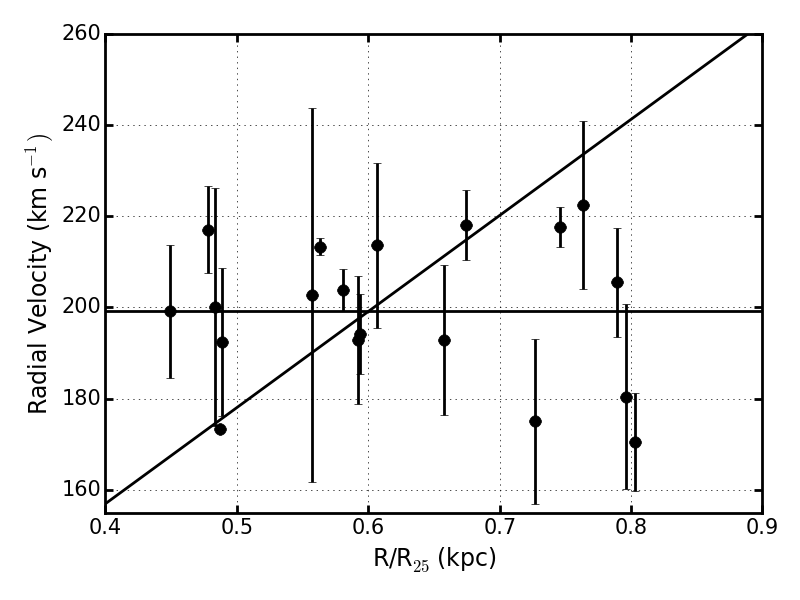
\includegraphics[width=0.65\textwidth]{ngc55/NGC55-RvsRV}
 \caption[Radial velocities for KMOS targets shown against projected radius]{
 Radial velocities for the KMOS RSGs (black points) shown against projected radius from the centre of NGC\,55 as defined by the Two Micron All Sky Survey~\citep[2MASS;][]{2006AJ....131.1163S} scaled by $R_{25}$~=~16.2\,$\pm$\,0.4\,arcmin~\citep{1991rc3..book.....D}.
Blue points show data for $\sim$200 BSGs in NGC\,55 from~\citet[][shown with 50\% transparency to highlight densely populated areas]{2008A&A...485...41C} alongside the rotation curve of NGC\,55~\citep[black solid line;][]{1991AJ....101..447P}.}
 \label{fig:RvsRV}
\end{figure}

As the observed data is taken over four different epochs, the variability of each source can be assessed.
To assess variability, the variability criteria of~\citet{2012A&A...546A..73H} is employed, i.e.

\begin{equation}
  \left|\frac{RV_i - \mu}{\sigma_i}\right| > 4.0,\label{eq:vary}
\end{equation}

\noindent where $RV_i$ is the radial velocity with an associated uncertainty  $\sigma_i$ measured on an individual night $i$ and $\mu$ is the average radial velocity for the target.
Using this criteria on all targets finds that none show compelling evidence for variability.
This adds strength to the suggestion that observed RSGs are intrinsically single objects as a result of the length of time spent as a RSG in a binary is significantly decreased (see discussion in Chapter~\ref{ch:ngc2100}).


% subsection radial_velocities (end)
\subsection{Stellar Parameters} % (fold)
\label{sub:stellar_parameters}

Stellar parameters are estimated for each target using the $J$-band analysis technique detailed in Chapter~\ref{ch:janal}.
This analyis is used to measure stellar parameters, including overall metallicity -- to a precision of $\pm$\,0.15\,dex at the resolution of KMOS observations with S/N~$\ge~100$.
The parameter ranges are given shown in Chapter~\ref{ch:janal}, Table~\ref{tb:mod_range}.

The analysis uses synthetic RSG spectra, extracted from {\sc marcs} model atmospheres~\citep{2008A&A...486..951G},
computed with corrections for non-local thermodynamic equilibrium for lines from titanium, iron, silicon and magnesium
\citep{2012ApJ...751..156B,2013ApJ...764..115B,2015ApJ...804..113B}.
The synthetic spectra are compared with observations using the $\chi$-squared statistic and the synthetic spectra are degraded to the resolution and sampling of the observations.

Estimated stellar parameters are listed in Table~\ref{tb:ngc55fit-pars} and the best-fit model spectra are shown with the final reduced science spectra in Figure~\ref{fig:ngc55spec}.
Assuming no spatial variations in metallicity the average metallicity of of the sample is $-$0.36\,$\pm$\,0.25\,dex.
This average value compares well to the average metallicity measured using 12 BSGs in NGC\,55 from~\citep[$-$0.4\,$\pm$\,0.13]{2012A&A...542A..79C}.
These authors find no evidence for spatial variations in metallicity in NGC\,55.

Kudritzki et al. (in prep) measure metallicities for $\sim$60 BSGs in NGC\,55 covering a larger spatial extent.
Combining all of the available data sets for BSGs and RSGs yields a metallicity gradient of $-$0.41\,$\pm$\,0.02\,dex/kpc: the first detected in this galaxy.
In order to independently calibrate this gradient with only RSGs would require a larger sample covering the full spatial profile of NGC\,55.

Figure~\ref{fig:ngc55ZvsR} displays the estimated metallicities shown as a function of the de-projected radial distance from the centre of the galaxy as defined by the Two Micron All Sky Survey~\citep[2MASS;][]{2006AJ....131.1163S}.
As in Figure~\ref{fig:RvsRV}, the de-projected radius is calculated by assuming a geometrical model with an inclination angle $i$~=~78\,\textdegree and a position angle $\phi$~=~109\,\textdegree~\citep{1991AJ....101..447P}.


% Using a maximum likelihood MCMC parameter estimation for a linear fit to the metallicities measured for RSGs in NGC\,55 I find (thus far) no evidence for spatial variations in metallicity, however, this is unsurprising given the spatial coverage and uncertainties associated with the measurements.
% In order to more accurately assess spatial variations in metallicity one would require a larger sample covering the full spatial profile of NGC\,55.


\begin{table*}
\begin{center}
\caption{Physical parameters determined for the KMOS targets in NGC\,55.\label{tb:ngc55fit-pars}}
\scriptsize
\begin{threeparttable}
\begin{tabular}{lr ccccl}
 \hline
 \hline
  Target  & IFU & $\xi$ (\kms) & [Z] & log\,$g$ & T$_{\rm eff}$ (K) & Notes\\
  \hline

% NGC55-RSG19 & 6 & 4.0\,$\pm$\,0.4 & $-$0.10\,$\pm$\,0.09 &\pp0.12\,$\pm$\,0.10 & 4260\,$\pm$\,80\o\\
NGC55-RSG24 &10 & 4.2\,$\pm$\,0.6 & $-$0.43\,$\pm$\,0.24 &$-$0.37\,$\pm$\,0.75 & 4180\,$\pm$\,330\\
NGC55-RSG25 & 8 & 3.2\,$\pm$\,0.9 & $-$0.53\,$\pm$\,0.33 &\pp0.12\,$\pm$\,0.36 & 3460\,$\pm$\,250\\
NGC55-RSG26 & 4 & 3.2\,$\pm$\,0.7 & $-$0.64\,$\pm$\,0.34 &\pp0.12\,$\pm$\,0.25 & 3560\,$\pm$\,280\\
NGC55-RSG35 &12 & 4.0\,$\pm$\,0.6 & $-$0.35\,$\pm$\,0.26 &$-$0.13\,$\pm$\,0.24 & 3750\,$\pm$\,120\\
NGC55-RSG39 &14 & 3.3\,$\pm$\,0.7 & $-$0.28\,$\pm$\,0.28 &$-$0.13\,$\pm$\,0.25 & 3700\,$\pm$\,100\\
NGC55-RSG43 &24 & 3.7\,$\pm$\,0.8 & $-$0.27\,$\pm$\,0.26 &\pp0.12\,$\pm$\,0.98 & 3960\,$\pm$\,250\\
NGC55-RSG57 & 1 & 4.0\,$\pm$\,0.7 & $-$0.39\,$\pm$\,0.28 &\pp0.10\,$\pm$\,0.24 & 3550\,$\pm$\,270\\
NGC55-RSG58 &15 & 3.5\,$\pm$\,0.7 & $-$0.38\,$\pm$\,0.27 &\pp0.12\,$\pm$\,0.96 & 3750\,$\pm$\,140\\
NGC55-RSG65 &17 & 4.2\,$\pm$\,0.5 & $-$0.25\,$\pm$\,0.19 &\pp0.11\,$\pm$\,0.97 & 3750\,$\pm$\,180\\
NGC55-RSG73 &19 & 3.2\,$\pm$\,0.5 & $-$0.26\,$\pm$\,0.15 &$-$0.86\,$\pm$\,0.50 & 3830\,$\pm$\,300\\

  \hline
  \end{tabular}
% \begin{tablenotes}

% \end{tablenotes}
  \end{threeparttable}
  \end{center}
\end{table*}

\begin{figure*}
 %\vspace{302pt}
 \begin{center}
 \centering
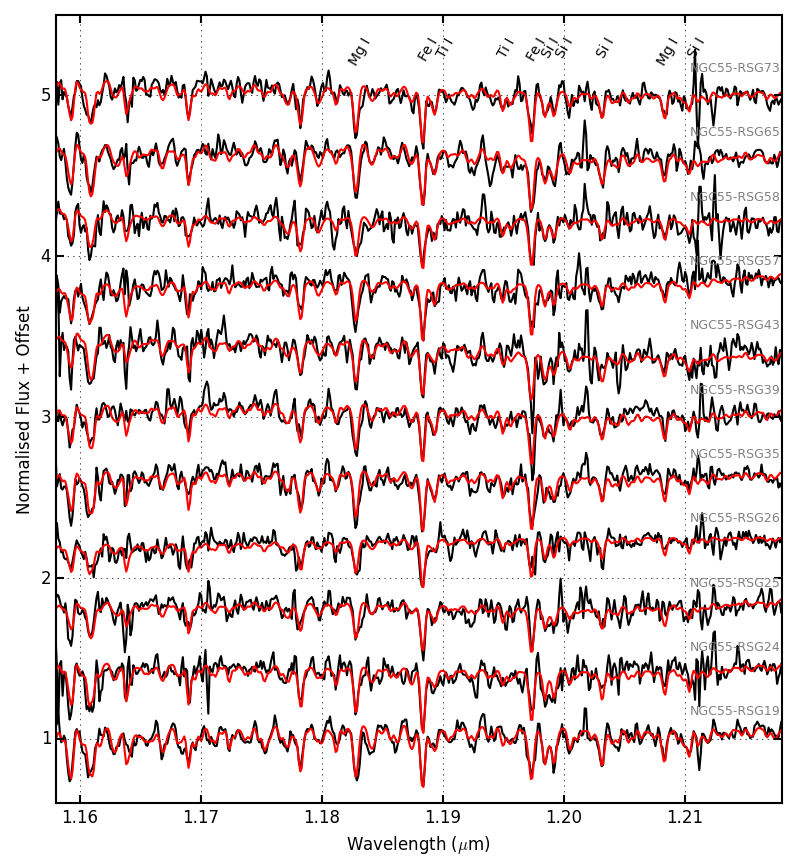
\includegraphics[width=0.75\textwidth]{ngc55/NGC55-model-fits}
\caption[Observed and best-fit model spectra of RSGs in NGC\,55]{Observed and best-fit model spectra of RSGs in NGC\,55 (black and red lines, respectively).
The lines used for the analysis, from left-to-right by species, are
Fe\,{\scriptsize I}$\,\lambda\lambda$1.188285,
1.197305;
Mg\,{\scriptsize I}$\,\lambda\lambda$1.182819,
1.208335;
Si\,{\scriptsize I}$\,\lambda\lambda$1.198419,
1.199157,
1.203151,
1.210353;
Ti\,{\scriptsize I}$\,\lambda\lambda$1.189289,
1.194954.\label{fig:ngc55spec}}
\end{center}
\end{figure*}


\begin{figure}
 \centering
 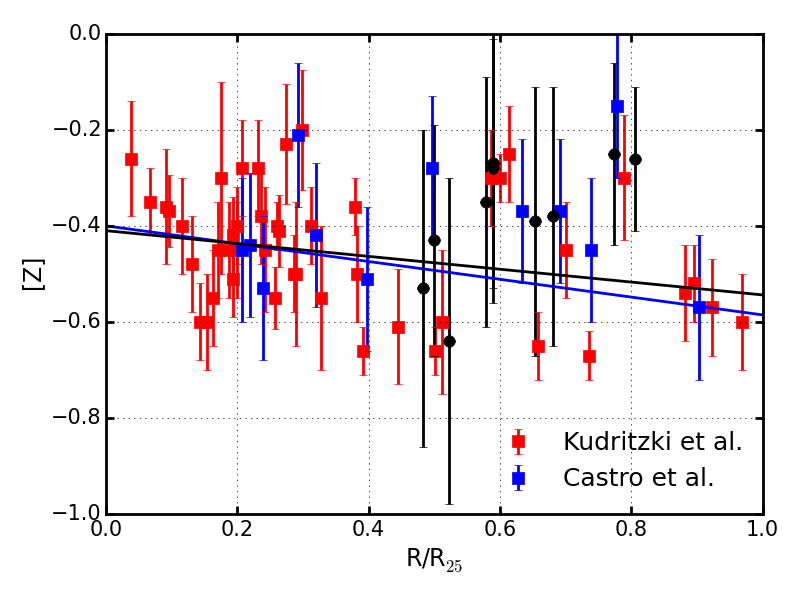
\includegraphics[width=0.65\textwidth]{ngc55/NGC55-ZvsR-BSGs}
 \caption[Metallicities for KMOS targets shown against de-projected radius]{
 Metallicities for KMOS RSGs (black points) shown against de-projected radius from the centre of NGC\,55 as defined by the Two Micron All Sky Survey~\citep{2006AJ....131.1163S} scaled by $R_{25}$~=~16.18\,arcmin~\citep{2004AJ....127.2031K}.
 The average metallicity of the KMOS RSGs is $-$0.36\,$\pm$\,0.25\,dex.
 Results for blue supergiant stars (BSGs)from Kudritzki et al. in prep. and~\citep{2012A&A...542A..79C} are shown with red and blue squares respectively.
Using a least squares fit to all of these measurements yields a metallicity gradient of $-$0.41\,$\pm$\,0.02\,dex/kpc (black line).
The blue line shows a least squares fit to just the BSG data.
 }
 \label{fig:ngc55ZvsR}
\end{figure}

Luminosities have been calculated for the targets using the bolometric corrections of~\citet{2013ApJ...767....3D} where the $F808$ HST bandpass where available,
otherwise the ground-based $I$-band filter has been used.
Figure~\ref{fig:ngc55-HRD} shows a H-R diagram for these targets using the temperatures estimated in Section~\ref{sec:ngc55results} along with SMC-like evolutionary tracks~\citep{2013A&A...558A.103G}.
Results for 15 RSGs in NGC\,300 (a fellow Sculptor galaxy also at $\sim$1.9\,Mpc) are shown in green on this figure for comparison~\citep{2015ApJ...805..182G}.
This appears to show a difference in the temperatures of the RSGs in the sample, however, we caution that the uncertainties on the temperatures presented in this study are significantly larger than those in~\citet{2015ApJ...805..182G}.

\begin{figure}
 \centering
 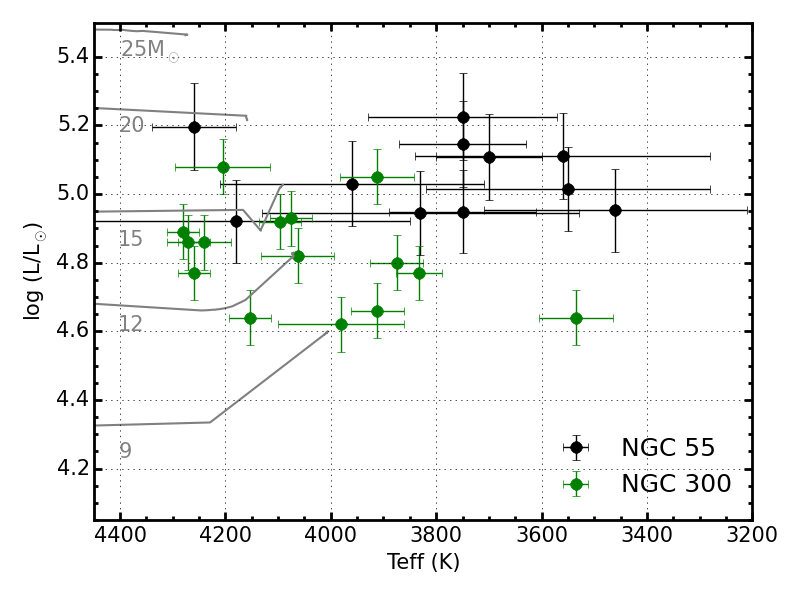
\includegraphics[width=0.65\textwidth]{ngc55/NGC55-HRD}
 \caption[Hertzsprung--Russell diagram for NGC\,55]{Hertzsprung--Russell diagram for NGC\,55.
Solid grey lines show SMC-like metallicity evolutionary models including rotation
\protect\citep{2013A&A...558A.103G}.
Results from~\cite{2015ApJ...805..182G} in NGC\,300 are shown in green for comparison.}
 \label{fig:ngc55-HRD}
\end{figure}

% subsection stellar_parameters (end)

% section results (end)

% \section{Discussion} % (fold)
% \label{sec:ngc55disc}

% \subsection{Orientation of NGC\,55} % (fold)
% \label{sub:orientation_of_ngc55}

% % subsection orientation_of_ngc55 (end)

% \subsection{Stellar Evolution} % (fold)
% \label{sub:stellar_evolution}

% Luminosities have been calculated for the targets using the bolometric corrections of~\citep{2013ApJ...767....3D} where the $F808$ HST bandpass where available,
% otherwise the ground-based $I$-band filter has been used.
% Figure~\ref{fig:ngc55-HRD} shows a H-R diagram for these targets using the temperatures estiamted in Section~\ref{sec:ngc55results} along with SMC-like evolutionary tracks~\citep{2013A&A...558A.103G}.


% \begin{figure}
%  \centering
%  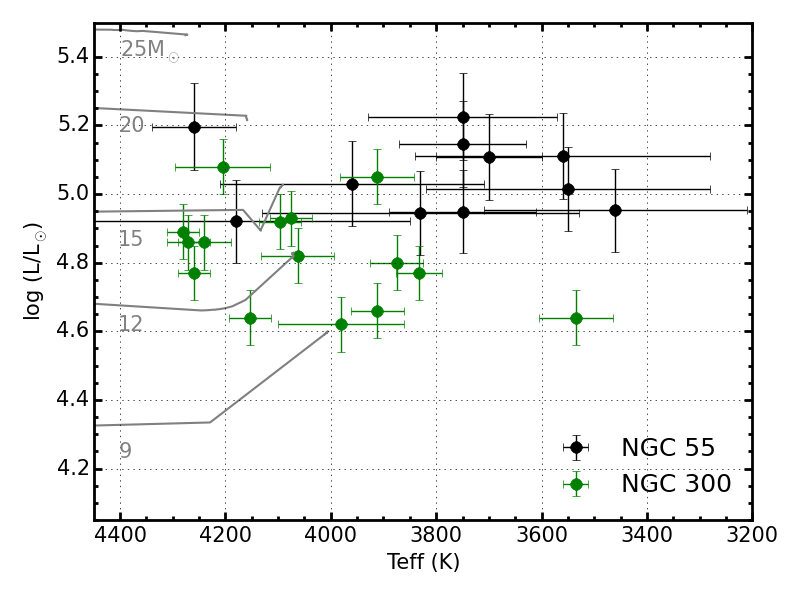
\includegraphics[width=0.65\textwidth]{ngc55/NGC55-HRD}
%  \caption[Hertzsprung--Russell diagram for NGC\,55]{Hertzsprung--Russell diagram for NGC\,55.
% Solid grey lines show SMC-like metallicity evolutionary models including rotation
% \protect\citep{2013A&A...558A.103G}.}
%  \label{fig:ngc55-HRD}
% \end{figure}

% subsection stellar_evolution (end)

% section discussion (end)

\section{Conclusions} % (fold)
\label{sec:ngc55conc}

I have presented multi-epoch near-IR spectroscopic observations of 22 RSGs in the Sculptor Group galaxy NGC\,55.
Radial velocities are presented and are shown to agree well with previous measurements in this galaxy, where all targets with reliable radial velocity measurements are consistent with membership to NGC\,55: confirming their nature as supergiants.
Variability is assessed for each target and I find no evidence for variability. A lack of variability is what one would expect from a sample consisting of single stars.

Stellar parameters are estimated for 10 of the highest S/N targets in the sample using the $J$-band analysis method described in Chapter~\ref{ch:janal}.
The average metallicity of the sample is $-$0.36\,$\pm$\,0.25, in good agreement with previous results.
No evidence is found for spatial variations in metallicity given the present sample, however, we note that this is expected as a result of the combination of the spatial coverage of the sample and the uncertainties in the metallicity parameter.
Luminosities are calculated and are compared with RSGs in NGC\,300 (a fellow Sculptor galaxy at $\sim$1.9\,Mpc) where there appears to be slight differences in the average effective temperatures of the two samples.


% section conclusions (end)

% \bibliography{../journals,../books}